\documentclass[12pt, a4paper]{article}

\usepackage[utf8]{inputenc}
\usepackage[greek, english]{babel}
\usepackage{alphabeta}
\usepackage{libertine}
\usepackage{graphicx}
\usepackage{biblatex}[sorting=nty] % sort alphabetically
\usepackage[table]{xcolor}
\usepackage{mathptmx} % Times New Roman
\usepackage{makecell}
\usepackage{setspace}
\usepackage{geometry}

\pagenumbering{arabic}
\onehalfspacing % Set line spacing to 1.5
\graphicspath{ {./output/} }
\addbibresource{refs.bib}

\def\code#1{\texttt{#1}}

\title{\Huge Probability and statistics for data analysis\\ \LARGE 2nd Assignment }


\begin{document}
	
	\begin{titlepage}
		\maketitle
		\begin{center}
			
			\LARGE Professors: I. Vrontos
			
			\large Athens University of Economics and Business
			
			\large MSc in Data Science
			
		\end{center}
		
	\end{titlepage}
	
	\tableofcontents
	\newpage
	
	\section{ANOVA Testing}
	
	\subsection{One-way ANOVA Tests}
	
	The relationship between $W$ and $Y, X1, X2, X3, X4$ can be found in Figure \ref{fig::boxplots_1}. Specifically:
	
	\begin{itemize}
		\item There are significant differences between X1 and W  on a $90\%$ confidence level $p = 0.0915$. The normality assumptions hold on a $95\%$ confidence level (S-W $p=0.268$, K-S $p=0.1506$) and so does the homogeneity assumption (Lev $p=0.3367$).
		
		\item There are no statistically significant differences between X2 and W  on a $90\%$ confidence level $p = 0.128$. The normality assumptions hold on a $95\%$ confidence level (S-W $p=0.8049$, K-S $p=0.2343$) and so does the homogeneity assumption (Lev $p=0.3412$).
		
		\item There are no statistically significant differences between X3 and W  on a $90\%$ confidence level $p = 0.876$. The normality assumptions hold on a $95\%$ confidence level (S-W $p=0.2555$, K-S $p=0.1112$). We reject the homogeneity assumption on a $90\%$ confidence level (Lev $p=0.0007$) and as such our results may not be accurate.
		
		\item There are statistically significant differences between X2 and W on a $95\%$ confidence level $p = 0.0168$. The normality assumptions hold on a $95\%$ confidence level (S-W $p=0.4243$, K-S $p=0.4261$) and so does the homogeneity assumption (Lev $p=0.4261$).
		
	\end{itemize}
	 
	
	\begin{figure}
		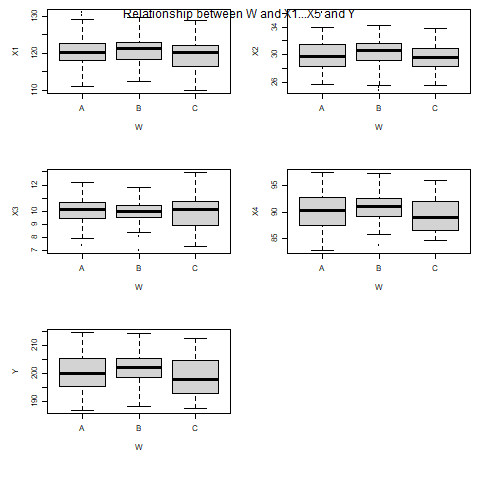
\includegraphics[width=8cm]{boxplots_1.png}
		\centering
		\caption{Boxplots of W in relation to the other variables.}
		\label{fig::boxplots_1}
	\end{figure}
	
	
	\subsection{Graphical Representation of $X_i$ effect on Y depending on W}
	
	Figure \ref{fig::scatterplot_1} shows the relation of Y with the other variables $X_i, i=1,2,3,4$ depending on W.
	
	\begin{figure}
		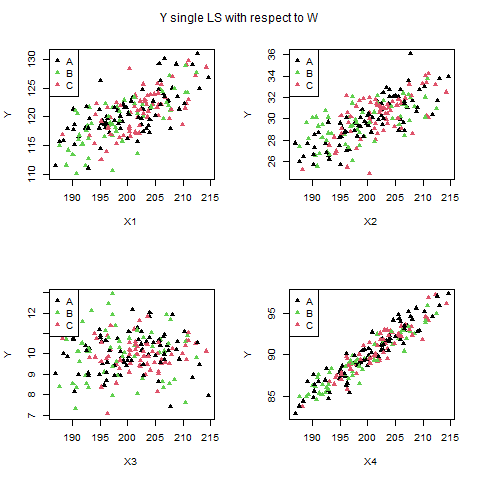
\includegraphics[width=8cm]{scatterplot_1.png}
		\centering
		\caption{Scatter-plot of Y and $X_i i=1,2,3,4$ depending on W.}
		\label{fig::scatterplot_1}
	\end{figure}
	
	
	\subsection{Simple Regression}
	
	Table \ref{tab::simple_1} shows the basic model where $Y = \beta_1 X4 + \beta_0 + \epsilon, \epsilon \sim N(0, \sigma^2)$.
	
	
% Table created by stargazer v.5.2.3 by Marek Hlavac, Social Policy Institute. E-mail: marek.hlavac at gmail.com
% Date and time: Sat, Dec 23, 2023 - 11:59:38 AM
\begin{table}[!htbp] \centering 
  \caption{Linear Regression of Y depending on X4} 
  \label{tab::simple_1} 
\begin{tabular}{@{\extracolsep{5pt}}lc} 
\\[-1.8ex]\hline 
\hline \\[-1.8ex] 
 & \multicolumn{1}{c}{\textit{Dependent variable:}} \\ 
\cline{2-2} 
\\[-1.8ex] & Y \\ 
\hline \\[-1.8ex] 
 X4 & 1.935$^{***}$ \\ 
  & p = 0.000 \\ 
  Constant & 26.197$^{***}$ \\ 
  & p = 0.00000 \\ 
 \hline \\[-1.8ex] 
Observations & 200 \\ 
R$^{2}$ & 0.886 \\ 
Adjusted R$^{2}$ & 0.886 \\ 
Residual Std. Error & 2.129 (df = 198) \\ 
F Statistic & 1,540.022$^{***}$ (df = 1; 198) \\ 
\hline 
\hline \\[-1.8ex] 
\textit{Note:}  & \multicolumn{1}{r}{$^{*}$p$<$0.1; $^{**}$p$<$0.05; $^{***}$p$<$0.01} \\ 
\end{tabular} 
\end{table} 

	
	
	\subsection{Multiple Regression}
	
	Table \ref{tab::multi_full_1} shows the full model  with base effects and interactions.
	
	
% Table created by stargazer v.5.2.3 by Marek Hlavac, Social Policy Institute. E-mail: marek.hlavac at gmail.com
% Date and time: Sat, Dec 23, 2023 - 11:59:38 AM
\begin{table}[!htbp] \centering 
  \caption{Mutiple Linear Regression of Y with main effects and interaction} 
  \label{tab::multi_full_1} 
\begin{tabular}{@{\extracolsep{5pt}}lc} 
\\[-1.8ex]\hline 
\hline \\[-1.8ex] 
 & \multicolumn{1}{c}{\textit{Dependent variable:}} \\ 
\cline{2-2} 
\\[-1.8ex] & Y \\ 
\hline \\[-1.8ex] 
 X1 & 1.168$^{***}$ \\ 
  & p = 0.00001 \\ 
  WB & $-$8.239 \\ 
  & p = 0.481 \\ 
  WC & $-$24.413$^{**}$ \\ 
  & p = 0.025 \\ 
  X2 & 2.701$^{***}$ \\ 
  & p = 0.00000 \\ 
  X3 & 0.322 \\ 
  & p = 0.166 \\ 
  X4 & $-$0.586 \\ 
  & p = 0.245 \\ 
  X1:WB & $-$0.212 \\ 
  & p = 0.538 \\ 
  X1:WC & $-$0.439 \\ 
  & p = 0.227 \\ 
  WB:X2 & $-$0.923 \\ 
  & p = 0.201 \\ 
  WC:X2 & $-$1.356$^{*}$ \\ 
  & p = 0.068 \\ 
  WB:X3 & 0.284 \\ 
  & p = 0.450 \\ 
  WC:X3 & $-$0.309 \\ 
  & p = 0.317 \\ 
  WB:X4 & 0.657 \\ 
  & p = 0.335 \\ 
  WC:X4 & 1.348$^{*}$ \\ 
  & p = 0.057 \\ 
  Constant & 28.361$^{***}$ \\ 
  & p = 0.0002 \\ 
 \hline \\[-1.8ex] 
Observations & 200 \\ 
R$^{2}$ & 0.917 \\ 
Adjusted R$^{2}$ & 0.911 \\ 
Residual Std. Error & 1.879 (df = 185) \\ 
F Statistic & 146.212$^{***}$ (df = 14; 185) \\ 
\hline 
\hline \\[-1.8ex] 
\textit{Note:}  & \multicolumn{1}{r}{$^{*}$p$<$0.1; $^{**}$p$<$0.05; $^{***}$p$<$0.01} \\ 
\end{tabular} 
\end{table} 

	
	
	\subsection{Checking the Full Model Assumptions}
	
	The model suffers from multi-collinearity ($GVIF > 10$) on most variables, meaning the model cannot be interpreted. We remove the variables with the biggest VIF scores and thus produce the model found in Table \ref{tab::multi_fixed_1}.
	
	We do not reject the normality assumption on the new model on a $95\%$ confidence level (S-W $p=0.2253$, K-S $p=0.5005$) nor the homogeneity assumption (Lev $p=0.2985$, Bart $p=0.4587$). Therefore the LS regression assumptions hold.
	
 	
% Table created by stargazer v.5.2.3 by Marek Hlavac, Social Policy Institute. E-mail: marek.hlavac at gmail.com
% Date and time: Sat, Dec 23, 2023 - 11:59:39 AM
\begin{table}[!htbp] \centering 
  \caption{Mutiple Linear Regression with no multicolinearity issues } 
  \label{tab::multi_fixed_1} 
\begin{tabular}{@{\extracolsep{5pt}}lc} 
\\[-1.8ex]\hline 
\hline \\[-1.8ex] 
 & \multicolumn{1}{c}{\textit{Dependent variable:}} \\ 
\cline{2-2} 
\\[-1.8ex] & Y \\ 
\hline \\[-1.8ex] 
 X1 & 0.968$^{***}$ \\ 
  & p = 0.000 \\ 
  X2 & 1.939$^{***}$ \\ 
  & p = 0.000 \\ 
  X3 & 0.245$^{*}$ \\ 
  & p = 0.077 \\ 
  X4 & 0.058 \\ 
  & p = 0.839 \\ 
  WB & 0.654$^{**}$ \\ 
  & p = 0.045 \\ 
  WC & 0.340 \\ 
  & p = 0.319 \\ 
  Constant & 17.944$^{***}$ \\ 
  & p = 0.0002 \\ 
 \hline \\[-1.8ex] 
Observations & 200 \\ 
R$^{2}$ & 0.909 \\ 
Adjusted R$^{2}$ & 0.907 \\ 
Residual Std. Error & 1.924 (df = 193) \\ 
F Statistic & 322.679$^{***}$ (df = 6; 193) \\ 
\hline 
\hline \\[-1.8ex] 
\textit{Note:}  & \multicolumn{1}{r}{$^{*}$p$<$0.1; $^{**}$p$<$0.05; $^{***}$p$<$0.01} \\ 
\end{tabular} 
\end{table} 

 	
 	
 	\subsection{Stepwise Model Selection}
	
	We use the stepwise selection procedure with the full model being the valid model presented in Table \ref{tab::multi_fixed_1}.
	
	The resulting model can be found in Table \ref{tab::multi_optimal_1}. Note that the dimensionality of the model has been reduced by 1 (removed X4) and that almost all terms are statistically significant on a $95\%$ confidence level.
	
	The model presents no multi-colinearity issues. We do not reject the normality assumption on the new model on a $95\%$ confidence level (S-W $p=0.2006$, K-S $p=0.6342$) nor the homogeneity assumption (Lev $p=0.4434$, Bart $p=0.4434$). Therefore the LS regression assumptions hold.
	
	
% Table created by stargazer v.5.2.3 by Marek Hlavac, Social Policy Institute. E-mail: marek.hlavac at gmail.com
% Date and time: Sat, Dec 23, 2023 - 12:04:21 PM
\begin{table}[!htbp] \centering 
  \caption{Stepwise Mutiple Linear Regression on Y} 
  \label{tab::multi_optimal_1} 
\begin{tabular}{@{\extracolsep{5pt}}lc} 
\\[-1.8ex]\hline 
\hline \\[-1.8ex] 
 & \multicolumn{1}{c}{\textit{Dependent variable:}} \\ 
\cline{2-2} 
\\[-1.8ex] & Y \\ 
\hline \\[-1.8ex] 
 X1 & 0.997$^{***}$ \\ 
  & p = 0.000 \\ 
  X2 & 1.999$^{***}$ \\ 
  & p = 0.000 \\ 
  X3 & 0.251$^{*}$ \\ 
  & p = 0.064 \\ 
  WB & 0.655$^{**}$ \\ 
  & p = 0.045 \\ 
  WC & 0.337 \\ 
  & p = 0.322 \\ 
  Constant & 17.878$^{***}$ \\ 
  & p = 0.0002 \\ 
 \hline \\[-1.8ex] 
Observations & 200 \\ 
R$^{2}$ & 0.909 \\ 
Adjusted R$^{2}$ & 0.907 \\ 
Residual Std. Error & 1.919 (df = 194) \\ 
F Statistic & 389.128$^{***}$ (df = 5; 194) \\ 
\hline 
\hline \\[-1.8ex] 
\textit{Note:}  & \multicolumn{1}{r}{$^{*}$p$<$0.1; $^{**}$p$<$0.05; $^{***}$p$<$0.01} \\ 
\end{tabular} 
\end{table} 

	
	
	\subsection{Estimating Y}
	
	When $X1=120, X2=30, X3=10, X4=90, W=B$ the stepwise model presented in Table \ref{tab::multi_optimal_1} predicts a value of $Y=200.6143$ with a $95\%$ confidence interval of $(200.1456 \leq Y \leq 201.083)$.
	
	
	\subsection{Categorizing Continuous Variable}
	The contingency table can be found in \ref{fig::contigency_1}.
	
	Executing the two-way ANOVA test between Y and W*Z, we determine that there are statistically significant differences in the means of Y depending on the two variables on a $95\%$ confidence interval (W: $p=5.12e-09$, Z: $p=0$) but not their interaction (W:Z $p= 0.305$). Therefore while the means deviate, the slope of Y to Z and Y to W does not change.
	
	We do not reject the normality assumption on the ANOVA test on a $95\%$ confidence level (S-W $p=0.8318$, K-S $p=0.9147$) nor the homogeneity assumption (Lev $p=0.6634$). Therefore the ANOVA assumptions hold.
	
	\begin{figure}
		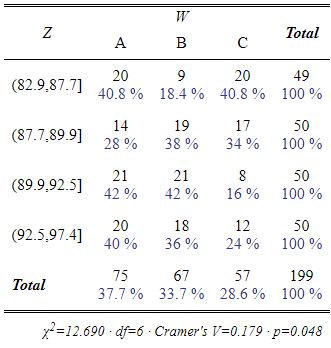
\includegraphics[width=8cm]{contigency_1.png}
		\centering
		\caption{Contingency table between W and Z (quantiles of X4)}
		\label{fig::contigency_1}
	\end{figure}
	
	
	\section{Explaining Weight Loss}
	
	
	\subsection{Exploring weight loss by workout and diet}
	
	The boxplots of Y depending on diet, workout and their interaction, can be found in Figure \ref{fig::boxplot_2}.
	
	\begin{figure}
		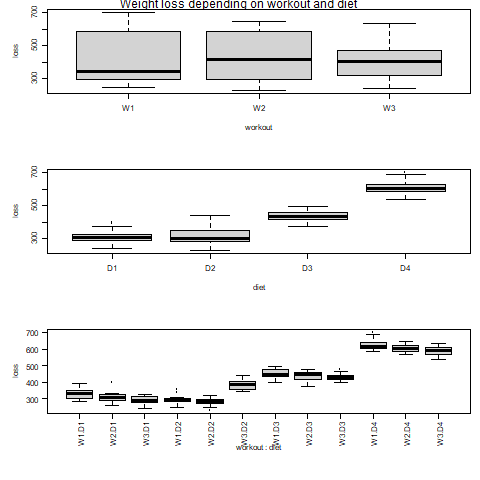
\includegraphics[width=10cm]{boxplot_2.png}
		\centering
		\caption{Boxplots of Y depending on diet, workout and their interaction. "W" denotes the workout level and "D" the diet level.}
		\label{fig::boxplot_2}
	\end{figure}
	
	
	\subsection{Weight loss depending on workout}
	
	Before we begin, we must check the parametric ANOVA assumptions. We reject the normality assumption (S-W $p=0$, K-S $p=0$) and the homogeneity assumption (Lev $p=0.0375$) on the same confidence level. Therefore the ANOVA assumptions do not hold and we need to use a non-parametric ANOVA test.

	We run a non-parametric ANOVA test on weight loss depending on the diet. The ANOVA model may be described as $$
	weightloss = \beta_1 Workout_2 + \beta_2 Workout_3 + \beta_0 + \epsilon, \epsilon \sim N(0, \sigma^2)
	$$
	where $Workout_2, Workout_3$ denote the workout level of the subject. Note that Workout Category 1 has been merged with the constant $\beta_0$.
	
	In our case
	$$
	weightloss = 17.094 Workout_2 + 2.675 Workout_3 + 413.6
	$$
	meaning that:
	
	\begin{itemize}
		\item if the subject belongs to the workout category 1, they will have on average a weight loss of $413.6$ calories per day.
		
		\item if the subject belongs to the workout category 2, they will have on average a weight loss of $413.6 + 17.094 = 430.694$ calories per day.
		
		\item if the subject belongs to the workout category 3, they will have on average a weight loss of $413.6 + 2.675 = 416.275$ calories per day.
	\end{itemize}
	
	However, we find no statistically significant differences in means on a $95\%$ confidence level (K-W $p=0.8194$), meaning that we should assume the model is in reality modeled as $weightloss = 413.6$. Additionally, we still reject the  homogeneity assumption on the same confidence level, therefore the ANOVA assumptions still do not hold and our analysis may be deficient.
	
	
	\subsection{Is workout significant?}
	
	As explained above, the differences between the means of any of the different workout categories (levels) can not be assumed to be significant.
	
	
	\subsection{Weight loss depending on the diet}
	
	We once again check the parametric ANOVA assumptions. We reject the normality assumption (S-W $p=0.0001$, K-S $p=0.0052$) and the homogeneity assumption (Lev $p=0.00011$) on the same confidence level. Therefore the ANOVA assumptions do not hold and we need to use a non-parametric ANOVA test.
	
	We run a non-parametric ANOVA test on weight loss depending on the diet. The model may be described as 
	$$
	weightloss = \beta_1 Diet_2 + \beta_2 Diet_3 + \beta_3 Diet_4 + \beta_0 + \epsilon, \epsilon \sim N(0, \sigma^2)
	$$
	where $Diet_2, Diet_3, Diet_4$ denote the diet category of the subject. Note that Diet Category 1 has been merged with the constant $\beta_0$.
	
	In our case,
	$$
	weightloss = 9.412 Diet_2 + 128.105 Diet_3 + 297.753 Diet_4 + 308.703
	$$
	meaning that:
	
	\begin{itemize}
		\item if the subject belongs to Diet Category 1, they will have on average a weight loss of $308.703$ calories per day.
		
		\item if the subject belongs to the Diet Category 2, they will have on average a weight loss of $308.703 + 9.412 = 318.115$ calories per day.
		
		\item if the subject belongs to the Diet Category 3, they will have on average a weight loss of $308.703 + 128.105 = 436.808$ calories per day.
		
		\item if the subject belongs to the Diet Category 4, they will have on average a weight loss of $308.703 + 297.753 = 606.456$ calories per day.
	\end{itemize}
	
	In this case, the difference in means on a $95\%$ confidence level are statistically significant (K-W $p=0$). However, we still reject the  homogeneity assumption, therefore the ANOVA assumptions still do not hold and our analysis may be deficient.
	
	
	\subsection{Is diet significant?}
	
	While there are differences in the means between different Diet Categories not all may be significant. Since we had to use a non-parametric ANOVA test because of the violation of the normality assumption, we will be using the "Dunn Kruskal-Wallis Multiple Comparison" as a non-parametric post-hoc test.
	
	We find that all groups have statistically significant differences in means on a $95\%$ significance level (Dunn $p<0.0001$) except from the differences between Diet 1 and Diet 2 (Dunn $p=0.8$). Thus, Diet 1 may not be a significant treatment.
	
	
	\subsection{Excluding the non-significant treatment}
	
	By eliminating Diet Category 1 from our dataset we end up with the model $weightloss = 118.694 Diet_3 + 288.341 Diet_4 + 318.115$. The differences in means are statistically significant on a $95\%$ confidence level (K-W $p=0$). 
	
	We use a non-parametric ANOVA test since we reject the normality assumption (S-W $p=0.0001$, K-S $p=0.0052$) and the homogeneity assumption (Lev $p=0.00011$) on the same confidence level. 
	
	
	\subsection{Two-way ANOVA on main effects}
	
	We use a parametric ANOVA test since there are very few alternatives for non-parametric Two-way ANOVA tests \cite{non_param_anova}. Our model can be found in Table \ref{tab::main_2} and can be described as
	
	$$
	weightloss = \alpha_1 Workout_2 + \alpha_2 Workout_3 + \beta_3 Diet_2 + \beta_4 Diet_3 + \beta_5 Diet_4 + \mu + \epsilon, \epsilon \sim N(0, \sigma^2)
	$$
	
	where $Workout_2, Workout_3$ denote the workout level and $Diet_2, Diet_3, Diet_4$ denote the diet category of the subject.  Note that Diet Category 1 and Workout Category 1 have been merged with the constant $\beta_0$.
	
	In our case, 
	$$
	weightloss = - 13.4910 Workout_2 - 0.6886  Workout_3 + 9.7644 Diet_2 + 130.0720 Diet_3 + 299.4477 Diet_4 + 312.7557
	$$ 
	meaning that:
	
	\begin{itemize}
		\item if the subject belongs to Workout Category 1 and Diet Category 1, they will on average experience a weight loss of $312.7557$ calories per day. 
		
		\item if the subject belongs to Diet Category 2, they will have on average an additional weight loss of $9.7644$ calories per day.
		
		\item if the subject belongs to Diet Category 3, they will have on average an additional weight loss of $130.0720$ calories per day.
		
		\item if the subject belongs to Diet Category 4, they will have on average an additional weight loss of $299.4477$ calories per day.
		
		\item if the subject belongs to Workout Category 2, they will have on average a reduction of weight loss (weight gain) of $13.4910$ calories per day.
		
		\item if the subject belongs to Workout Category 3, they will have on average a reduction of weight loss (weight gain) of $0.6886$ calories per day.
	\end{itemize}
	
	We reject the normality assumption on a $95\%$ confidence level (S-W $p=0.0004$, K-S $p=0.01525$) but not the homogeneity assumption (Lev $p=0.2821$, Bart $p=0.3741$) on the same confidence level. Therefore the ANOVA assumptions do not hold and our analysis may be deficient, since we can not use a non-parametric test in this case.
	
	
% Table created by stargazer v.5.2.3 by Marek Hlavac, Social Policy Institute. E-mail: marek.hlavac at gmail.com
% Date and time: Sat, Dec 23, 2023 - 8:07:23 PM
\begin{table}[!htbp] \centering 
  \caption{Two-Way ANOVA between weight loss and main effects} 
  \label{tab::main_2} 
\begin{tabular}{@{\extracolsep{5pt}}lc} 
\\[-1.8ex]\hline 
\hline \\[-1.8ex] 
 & \multicolumn{1}{c}{\textit{Dependent variable:}} \\ 
\cline{2-2} 
\\[-1.8ex] & loss \\ 
\hline \\[-1.8ex] 
 workoutW2 & $-$13.491$^{**}$ \\ 
  & p = 0.021 \\ 
  workoutW3 & $-$0.689 \\ 
  & p = 0.907 \\ 
  dietD2 & 9.764 \\ 
  & p = 0.132 \\ 
  dietD3 & 130.072$^{***}$ \\ 
  & p = 0.000 \\ 
  dietD4 & 299.448$^{***}$ \\ 
  & p = 0.000 \\ 
  Constant & 312.756$^{***}$ \\ 
  & p = 0.000 \\ 
 \hline \\[-1.8ex] 
Observations & 240 \\ 
R$^{2}$ & 0.926 \\ 
Adjusted R$^{2}$ & 0.925 \\ 
Residual Std. Error & 35.958 (df = 234) \\ 
F Statistic & 589.737$^{***}$ (df = 5; 234) \\ 
\hline 
\hline \\[-1.8ex] 
\textit{Note:}  & \multicolumn{1}{r}{$^{*}$p$<$0.1; $^{**}$p$<$0.05; $^{***}$p$<$0.01} \\ 
\end{tabular} 
\end{table} 

	
	
	\subsection{Excluding non-significant treatments}
	We will be using the parametric TukeyHSD test, as there are no good non-parametric alternatives. All main effects seem to be statistically significant on a $95\%$ confidence level, apart from D2-D1 ($p=0.49$) and W3-W1 ($p=0.88$).
	
	By removing the non-statistically significant treatments we end up with the model 
	$$
	weightloss = -15.171 Workout_2 + 155.623 Diet_3 + 325.854 Diet_4 + 296.285 
	$$ 
	meaning that:
	
	\begin{itemize}
		\item if the subject belongs to Workout Categories 1 or 3 and Diet Categories 1 or 2, they will on average experience a weight loss of $296.285$ calories per day (their workout and/or diet do not significantly change the weight loss). 
		
		\item if the subject belongs to Diet Category 3, they will have on average an additional weight loss of $155.623$ calories per day.
		
		\item if the subject belongs to Diet Category 4, they will have on average an additional weight loss of $325.854$ calories per day.
		
		\item if the subject belongs to Workout Category 2, they will have on average a reduction of weight loss (weight gain) of $15.171$ calories per day.

	\end{itemize}
	
	We do not reject the normality assumption on a $95\%$ confidence level (S-W $p=0.7103$, K-S $p=0.7103$) nor the homogeneity assumption (Lev $p=0.6461$, Bart $p=0.7128$) on the same confidence level. Therefore the ANOVA assumptions hold. It therefore does appear that refocusing the model on the statistically important variables has fixed the normality issues previously encountered.
	
	
	\subsection{Two-way ANOVA including interactions}
	
	The two-way ANOVA model including main effects and their interactions can be found in Table \ref{tab::full_2}. We notice that 
	
	
% Table created by stargazer v.5.2.3 by Marek Hlavac, Social Policy Institute. E-mail: marek.hlavac at gmail.com
% Date and time: Sat, Dec 23, 2023 - 8:07:24 PM
\begin{table}[!htbp] \centering 
  \caption{Two-Way ANOVA between weight loss and main effects 
          including interactions} 
  \label{tab::full_2} 
\begin{tabular}{@{\extracolsep{5pt}}lc} 
\\[-1.8ex]\hline 
\hline \\[-1.8ex] 
 & \multicolumn{1}{c}{\textit{Dependent variable:}} \\ 
\cline{2-2} 
\\[-1.8ex] & loss \\ 
\hline \\[-1.8ex] 
 dietD2 & $-$34.299$^{***}$ \\ 
  & p = 0.00002 \\ 
  dietD3 & 122.159$^{***}$ \\ 
  & p = 0.000 \\ 
  dietD4 & 296.266$^{***}$ \\ 
  & p = 0.000 \\ 
  workoutW2 & $-$20.924$^{**}$ \\ 
  & p = 0.014 \\ 
  workoutW3 & $-$37.341$^{***}$ \\ 
  & p = 0.00001 \\ 
  dietD2:workoutW2 & 10.264 \\ 
  & p = 0.383 \\ 
  dietD3:workoutW2 & 7.374 \\ 
  & p = 0.598 \\ 
  dietD4:workoutW2 & 0.996 \\ 
  & p = 0.931 \\ 
  dietD2:workoutW3 & 129.327$^{***}$ \\ 
  & p = 0.000 \\ 
  dietD3:workoutW3 & 17.117 \\ 
  & p = 0.211 \\ 
  dietD4:workoutW3 & 0.852 \\ 
  & p = 0.941 \\ 
  Constant & 328.591$^{***}$ \\ 
  & p = 0.000 \\ 
 \hline \\[-1.8ex] 
Observations & 240 \\ 
R$^{2}$ & 0.961 \\ 
Adjusted R$^{2}$ & 0.959 \\ 
Residual Std. Error & 26.516 (df = 228) \\ 
F Statistic & 511.357$^{***}$ (df = 11; 228) \\ 
\hline 
\hline \\[-1.8ex] 
\textit{Note:}  & \multicolumn{1}{r}{$^{*}$p$<$0.1; $^{**}$p$<$0.05; $^{***}$p$<$0.01} \\ 
\end{tabular} 
\end{table} 

	
	We do not reject the normality assumption on a $95\%$ confidence level (S-W $p=0.4452$, K-S $p=0.7103$) nor the homogeneity assumption (Lev $p=0.3774$, Bart $p=0.4358$) on the same confidence level. Therefore the ANOVA assumptions hold. It would appear that including the interaction terms fixes the normality issues previously encountered.
		
		
		
	\subsection{Stepwise model selection}
	
	We use the stepwise selection procedure with the full model being the valid model presented in Table \ref{tab::full_2}.
	
	The selection does not return a different model by AIC, meaning that even the variables with non-statistically significant terms are necessary to keep AIC high.
	
	
	\subsection{Interaction between workout, diet and loss }
	
	Figure \ref{fig::interaction_2} displays the differences in means between weight loss and different workout and diet categories.
	
	We observe that Diet Category 2 is the only one with a significant interaction (with Workout Category 3), as indicated by the change of slope. Generally however, while there are significant deviations in the means of weight loss depending on the Diet, the same can not be said about the Workout (no slope), corroborating our previous analysis.
	
	\begin{figure}
		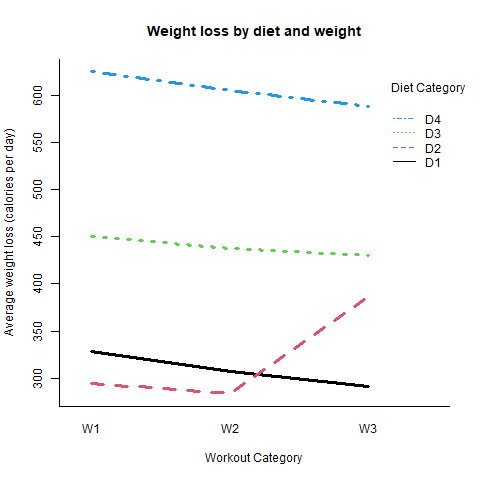
\includegraphics[width=10cm]{interaction_2.png}
		\centering
		\caption{Interaction plot of Two-way optimal ANOVA model, with the weight loss as the response, workout as the x-axis and diet as the trace variable.}
		\label{fig::interaction_2}
	\end{figure}
	
	
	\subsection{Comparison with the Null model}
	
	We use the \code{anova} R command to execute a Partial-F test between the null (constant) model and the model with main effects. We observe that the main effects model is statistically better than the null ($p=0$). In the same way we observe that the main effects model with interactions is also better than the null ($p=0$).
	
	\printbibliography
\end{document}